\documentclass[conference]{IEEEtran}
\IEEEoverridecommandlockouts

\usepackage{cite}
\usepackage{amsmath,amssymb,amsfonts}
\usepackage{graphicx}
\usepackage{textcomp}
\usepackage{xcolor}
\usepackage{booktabs}
\usepackage{float}
\usepackage[hidelinks]{hyperref}

\def\BibTeX{{\rm B\kern-.05em{\sc i\kern-.025em b}\kern-.08em
    T\kern-.1667em\lower.7ex\hbox{E}\kern-.125emX}}

\begin{document}

\title{Improving Robustness of Semantic Segmentation on Cityscapes using DeepLabV3 with a Pretrained ResNet-50 Backbone}

\author{\IEEEauthorblockN{Jochem Plegt}
\IEEEauthorblockA{\textit{Eindhoven University of Technology}}}

\maketitle

\begin{abstract}
Semantic segmentation in autonomous driving requires models that are not only accurate on clean benchmark data, but also robust under real-world image corruptions. This paper investigates whether replacing a baseline U-Net with a DeepLabV3 model using a pretrained ResNet-50 backbone, combined with data augmentation and cosine annealing learning rate scheduling, improves both segmentation performance and robustness on the Cityscapes dataset. To preserve the pretrained BatchNorm statistics, the backbone is frozen during training. Three hypotheses are formulated and evaluated through a systematic ablation study isolating the effects of architecture, random flip, and color jitter augmentation. Experiments show a modest improvement in clean-data performance (Mean Dice 0.4681 vs.\ 0.4598) and a substantially larger gain under common image corruptions (Mean Dice 0.4108 vs.\ 0.2079), corresponding to robustness retention of 87.8\% vs.\ 45.2\%. The ablation reveals that color jitter is the dominant robustness factor, outperforming random flip by $+0.035$ Mean Dice. A frozen-vs.-fine-tuned comparison further shows that the frozen backbone outperforms fine-tuning on robustness (0.4108 vs.\ 0.3901) despite nearly identical clean performance (0.4681 vs.\ 0.4668), providing stronger evidence that frozen ImageNet features may retain partial invariance to photometric corruptions.
\end{abstract}

\begin{IEEEkeywords}
Semantic Segmentation, DeepLabV3, ResNet-50, Transfer Learning, Data Augmentation, Robustness
\end{IEEEkeywords}

%% -------------------------------------------------------
\section{Introduction}

Semantic segmentation is a fundamental computer vision task in which a semantic label is assigned to every pixel in an image. In safety-critical applications such as autonomous driving, reliable segmentation is essential, since errors in scene understanding may propagate to downstream decision-making systems~\cite{grigorescu2020survey}. Unlike standard image classification, semantic segmentation requires both high-level semantic understanding and precise spatial localization at pixel level.

Deploying segmentation models in real-world driving scenarios remains challenging. Images acquired by autonomous vehicles are affected by illumination changes, weather conditions, blur, sensor noise, and other appearance shifts. As a result, a model that performs well on clean benchmark data may still fail under corrupted or shifted inputs. In this setting, robustness is as important as peak in-distribution performance.

A widely used baseline for semantic segmentation is U-Net~\cite{ronneberger2015unet}, an encoder-decoder architecture with skip connections that combine high-level semantic information with low-level spatial detail. This design is effective for dense prediction tasks, especially when training from scratch. However, when trained only on a fixed target dataset, such models may become sensitive to appearance variations that are not sufficiently represented during training.

DeepLabV3~\cite{chen2017deeplab} provides a stronger alternative by using atrous convolutions and atrous spatial pyramid pooling (ASPP) to capture multi-scale contextual information without aggressively reducing spatial resolution. This is particularly relevant for urban-scene segmentation, where objects and regions appear at multiple scales. When combined with a ResNet-50 backbone~\cite{he2016resnet} pretrained on ImageNet~\cite{russakovsky2015imagenet}, the model can exploit transferable visual representations learned from a large and diverse image collection. Transfer learning is widely used because pretrained models often provide a strong initialization or feature extractor, especially when labeled target data is limited.

Data augmentation further reduces the distribution gap between clean training images and corrupted test conditions, making it particularly relevant for robustness.

This motivates the following research question: \textit{does replacing the baseline U-Net with a DeepLabV3 model using a pretrained ResNet-50 backbone, combined with data augmentation, improve both segmentation performance and robustness to image corruptions on the Cityscapes dataset?}

To structure the investigation, three hypotheses are formulated prior to experimentation. \textbf{H1:} A pretrained ImageNet backbone encodes texture-aware visual representations that are partially invariant to appearance corruptions, since these features were learned from a large and diverse image collection. \textbf{H2:} Color jitter augmentation improves robustness by directly simulating brightness, contrast, and saturation corruptions during training, thereby reducing the distribution gap between clean training images and corrupted test images. \textbf{H3:} The pretrained backbone and augmentation provide complementary robustness gains, with augmentation expected to be the dominant contributor. A frozen-vs.-fine-tuned comparison is included to partially isolate the backbone contribution from architectural differences between U-Net and DeepLabV3.

To answer this question, a DeepLabV3-ResNet50 model is trained on Cityscapes~\cite{cordts2016cityscapes} and compared with a baseline U-Net on clean and corrupted test conditions. The ablation study in Section~\ref{sec:ablation} is used to evaluate the relative contribution of each factor and to assess the three hypotheses. The code used to produce the results presented in this paper is publicly available at: \url{https://github.com/JochemPlegt/5LSM0_NN_jochem}.

%% -------------------------------------------------------
\section{Related Work}

\subsection{Semantic Segmentation}
U-Net~\cite{ronneberger2015unet} is a widely used encoder-decoder segmentation architecture with skip connections that combine semantic context with low-level spatial detail. DeepLabV3~\cite{chen2017deeplab,chen2018deeplabv3plus} uses atrous convolutions and atrous spatial pyramid pooling (ASPP) to aggregate multi-scale context, which is well suited to urban-scene segmentation.

The Cityscapes dataset~\cite{cordts2016cityscapes} is a standard benchmark for semantic segmentation in autonomous driving. Because segmentation quality depends on overlap between predicted and ground-truth regions, overlap-based metrics such as Dice and IoU are generally more informative than plain pixel accuracy, especially in the presence of class imbalance and large dominant regions~\cite{maierhein2024metrics,reinke2024pitfalls}.

\subsection{Pretrained Backbones}
DeepLabV3 can be combined with a ResNet-50 backbone~\cite{he2016resnet} pretrained on ImageNet~\cite{russakovsky2015imagenet}. Residual connections enable effective optimization of deep networks, while pretraining provides general-purpose visual features that transfer well to downstream tasks. This fits the transfer-learning setting, in which knowledge from a source task is reused for a target task~\cite{oquab2014transfer}.

\subsection{Robustness}
Hendrycks and Dietterich~\cite{hendrycks2019robustness} introduced a benchmark for evaluating neural-network robustness under common image corruptions such as noise, blur, and weather effects. Their results show that models trained only on clean data can degrade substantially under corrupted inputs, which is especially problematic in safety-critical settings such as autonomous driving~\cite{grigorescu2020survey}.

Common corruptions represent a form of distribution shift, and data augmentation is a natural strategy for reducing the resulting performance gap by exposing the model to broader appearance variation during training.

\subsection{Texture Bias and Robustness}
Geirhos~et~al.~\cite{geirhos2019} demonstrated that ImageNet-trained CNNs exhibit a strong texture bias: when classifying images, these models rely primarily on local texture statistics rather than global shape information. Because texture-based representations encode local statistical patterns rather than precise pixel values, they are partially invariant to global appearance corruptions such as noise and color shift. A pretrained backbone that has learned texture-rich representations from ImageNet may therefore generalize better to corrupted inputs than a model trained exclusively on clean Cityscapes images, which motivates \textbf{H1}.

%% -------------------------------------------------------
\section{Methodology}

\subsection{Datasets and Preprocessing}
The Cityscapes dataset~\cite{cordts2016cityscapes} is used for training and validation, using the official fine-annotation splits: 2,975 training images and 500 validation images, across 19 semantic classes. All images are resized to $256 \times 256$ pixels to reduce computational cost, although this may remove fine-grained detail for small objects.

Images are normalized using the ImageNet mean $(0.485, 0.456, 0.406)$ and standard deviation $(0.229, 0.224, 0.225)$. During training, random horizontal flipping is applied jointly to images and masks, while color jitter is applied to the image before normalization. Augmentations are used only during training; no augmentation is applied at validation or test time.

\subsection{Model Architecture}
Two models are evaluated: a baseline U-Net and a DeepLabV3-ResNet50 model. The baseline U-Net uses a standard encoder-decoder structure with four downsampling and four upsampling stages and skip connections to improve localization.

The proposed model uses DeepLabV3 with a ResNet-50 backbone pretrained on ImageNet. DeepLabV3 uses atrous convolutions and an ASPP module to aggregate context at multiple receptive fields, which is well suited to urban-scene segmentation where objects appear at vastly different scales. The classifier head is replaced by a $1 \times 1$ convolution producing 19 output channels, and the auxiliary classifier is removed. All models are implemented in PyTorch.

To investigate \textbf{H1} directly, the backbone is used as a fixed feature extractor: all parameters are frozen and BatchNorm layers are kept in evaluation mode, so that only the classifier head is trained. This preserves the pretrained BatchNorm statistics and ensures the features remain in exactly the form learned on ImageNet. To isolate the contribution of the pretrained features, a fine-tuned variant is additionally evaluated in which all backbone parameters are allowed to update during training, using the same architecture and augmentation.

Color jitter perturbs brightness, contrast, saturation, and hue before normalization, directly simulating a subset of common photometric corruptions and forming the primary mechanism behind \textbf{H2}. Random horizontal flip is applied jointly to image and mask and does not alter appearance statistics. The ablation study in Section~\ref{sec:ablation} decomposes the contribution of each augmentation type separately.

\subsection{Training}
Both models are trained on the Cityscapes training split for 100 epochs using AdamW (weight decay $10^{-2}$), cross-entropy loss with ignore index 255 for void pixels, and a batch size of 64. The baseline U-Net is trained with a fixed learning rate of 0.001. The DeepLabV3-ResNet50 model uses the same initial learning rate together with cosine annealing scheduling ($T_{\max}=100$, $\eta_{\min}=0$). When color jitter is applied, brightness and contrast factors are sampled uniformly from $[0.7, 1.3]$, saturation from $[0.7, 1.3]$, and hue shift from $[-0.05, 0.05]$.

Model selection is based on validation loss; the test benchmark is reserved for final evaluation.

\subsection{Evaluation}
Model performance is evaluated on two benchmarks. For \textit{peak performance}, Mean Dice and Mean IoU are measured on the clean Cityscapes test set. For \textit{robustness}, the same metrics are measured on a corrupted test set containing common image corruptions such as noise, blur, and weather effects~\cite{hendrycks2019robustness}. Robustness retention is additionally defined as the ratio between corrupted and clean Mean Dice, providing a scale-independent measure of degradation under corruption.

Both benchmarks are evaluated through the challenge submission server.

%% -------------------------------------------------------
\section{Results}

\subsection{Peak Performance}

Table~\ref{tab:peak} reports the performance on the clean Cityscapes test set. The frozen DeepLabV3 achieves a Mean Dice of 0.4681 and Mean IoU of 0.3887, compared to 0.4598 and 0.3758 for the baseline U-Net. The fine-tuned variant achieves nearly identical clean performance (0.4668 Mean Dice), indicating that frozen and fine-tuned backbones differ primarily in robustness rather than in-distribution accuracy.

\begin{table}[h]
\centering
\caption{Peak performance on the clean Cityscapes test set.}
\label{tab:peak}
\begin{tabular}{lcc}
\toprule
Model & Mean Dice & Mean IoU \\
\midrule
Baseline U-Net          & 0.4598 & 0.3758 \\
DeepLabV3 (frozen)      & 0.4681 & 0.3887 \\
DeepLabV3 (fine-tuned)  & 0.4668 & 0.3871 \\
\bottomrule
\end{tabular}
\end{table}

\subsection{Robustness}

Table~\ref{tab:robustness} reports the results on the corrupted Cityscapes test set. The frozen DeepLabV3 achieves a Mean Dice of 0.4108, nearly doubling the baseline U-Net (0.2079), with a retention of 87.8\% vs.\ 45.2\%. The fine-tuned variant achieves 0.3901 Mean Dice (83.6\% retention), demonstrating that the frozen backbone provides greater robustness despite nearly identical clean performance (Table~\ref{tab:peak}).

\begin{table}[h]
\centering
\caption{Robustness results on the corrupted Cityscapes test set. Retention is defined as the ratio of corrupted to clean Mean Dice.}
\label{tab:robustness}
\begin{tabular}{lccc}
\toprule
Model & Mean Dice & Mean IoU & Retention (\%) \\
\midrule
Baseline U-Net         & 0.2079 & 0.1539 & 45.2 \\
DeepLabV3 (frozen)     & 0.4108 & 0.3358 & 87.8 \\
DeepLabV3 (fine-tuned) & 0.3901 & 0.3178 & 83.6 \\
\bottomrule
\end{tabular}
\end{table}

\begin{figure}[h]
    \centering
    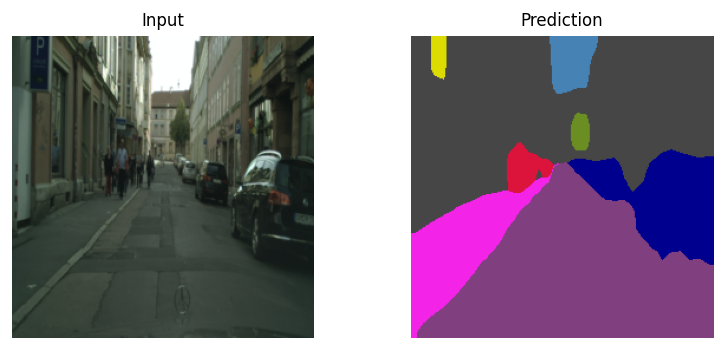
\includegraphics[width=\linewidth]{figures/deeplabv3_pred1.png}\\[3pt]
    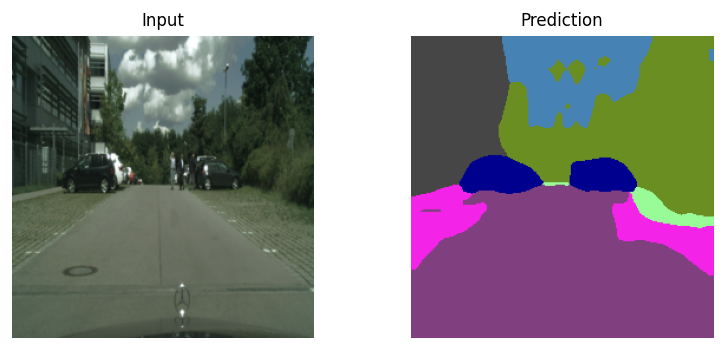
\includegraphics[width=\linewidth]{figures/deeplabv3_pred2.png}
    \caption{Segmentation predictions by DeepLabV3 (frozen) on the Cityscapes validation set. Each row shows the input image (left) and predicted semantic mask (right). Top: a typical successful prediction with accurate road, vegetation, and building segmentation. Bottom: a failure case in which pedestrians and traffic signs are missed at $256\times256$ resolution.}
    \label{fig:predictions}
\end{figure}

\begin{figure}[t]
    \centering
    
\includegraphics[width=\linewidth]{figures/robustness_per_category.png}
    \caption{Per-class Dice on the clean Cityscapes validation set, sorted by DeepLabV3 score. Large, texture-dominated classes (road, building, vegetation) score highest; small-object classes (person, rider, traffic sign) score lowest for both models.}
    \label{fig:per_category}
\end{figure}

The ablation study in Section~\ref{sec:ablation} decomposes this robustness gain and evaluates the three hypotheses.

\subsection{Ablation Study}
\label{sec:ablation}

To evaluate the three hypotheses and decompose the contributions of architecture and augmentation type to robustness, seven configurations were evaluated on the corrupted Cityscapes benchmark. Results are reported in Table~\ref{tab:ablation}.

\begin{table}[h]
\centering
\caption{Ablation study on the corrupted Cityscapes test set, isolating the effect of architecture and augmentation type on robustness.}
\label{tab:ablation}
\begin{tabular}{llcc}
\toprule
Model & Augmentation & Mean Dice & Mean IoU \\
\midrule
U-Net                  & None (baseline) & 0.2079 & 0.1539 \\
U-Net                  & Flip only       & 0.3136 & 0.2457 \\
U-Net                  & Jitter only     & 0.3490 & 0.2781 \\
U-Net                  & Flip + Jitter   & 0.3601 & 0.2883 \\
\midrule
DeepLabV3 (frozen)     & None            & 0.2261 & 0.1747 \\
DeepLabV3 (fine-tuned) & Flip + Jitter   & 0.3901 & 0.3178 \\
DeepLabV3 (frozen)     & Flip + Jitter   & \textbf{0.4108} & \textbf{0.3358} \\
\bottomrule
\end{tabular}
\end{table}

\textbf{Architecture vs.\ augmentation (H1, H2).}
Switching from U-Net to DeepLabV3 without augmentation yields only a modest improvement ($+0.018$ Mean Dice). By contrast, adding color jitter alone to the baseline U-Net produces a substantially larger gain ($+0.141$ Mean Dice), and adding random flip alone yields $+0.106$ Mean Dice. These results support \textbf{H2}: data augmentation is a considerably more effective robustness strategy than architectural change alone. To evaluate \textbf{H1} directly, a frozen-vs.-fine-tuned comparison was conducted using identical DeepLabV3 architecture and augmentation. The frozen backbone achieves $0.4108$ Mean Dice under corruption, compared to $0.3901$ for the fine-tuned backbone ($+0.021$), despite nearly identical clean performance ($0.4681$ vs.\ $0.4668$). This provides direct support for \textbf{H1}: the frozen pretrained features retain partial invariance to photometric corruptions that is reduced when the backbone is adapted to Cityscapes during training, consistent with the texture-bias account of ImageNet-pretrained CNNs~\cite{geirhos2019}.

\textbf{Jitter vs.\ flip (H2).}
Color jitter (0.3490) substantially outperforms random flip (0.3136), a difference of $+0.035$ Mean Dice, directly supporting \textbf{H2}. Color jitter perturbs brightness, contrast, saturation, and hue, directly simulating the photometric corruptions present at test time. Random flip does not alter appearance statistics and therefore does not reduce the photometric distribution gap. Combining both augmentations (0.3601) adds only a marginal gain over jitter alone ($+0.011$). This conclusion is based on a single aggregate corruption score; whether jitter also outperforms flip for structural corruptions such as blur cannot be determined from available results.

\textbf{Architecture and augmentation combined (H3).}
When augmentation is combined with DeepLabV3, performance reaches 0.4108 Mean Dice, exceeding both augmented U-Net (0.3601) and DeepLabV3 without augmentation (0.2261). The incremental gain of DeepLabV3 over augmented U-Net ($+0.051$) is larger than the gain without augmentation ($+0.018$), and the combined gain ($+0.203$) exceeds the sum of the individual contributions ($+0.170$). This numerical pattern is consistent with \textbf{H3}, but the design confounds architectural differences (ASPP, atrous convolutions) with backbone pretraining and training procedure (cosine annealing vs.\ fixed LR). The frozen-vs.-fine-tuned comparison partially disentangles these: the frozen backbone outperforms fine-tuning ($+0.021$ Mean Dice) under identical architecture and augmentation, providing cleaner evidence for the backbone contribution. Whether the backbone and augmentation interact synergistically or additively cannot be fully resolved from the available data.

%% -------------------------------------------------------
\section{Conclusion and Discussion}

The experiments show that robustness and clean-data accuracy respond very differently to the proposed changes: the clean-data gain is modest (Mean Dice $+0.0083$), while the robustness gain is substantial ($+0.2029$, retention 87.8\% vs.\ 45.2\%).

The ablation study provides a more precise picture of what drives this robustness gain. Color jitter augmentation is the dominant factor, outperforming random flip by $+0.035$ Mean Dice and accounting for most of the robustness improvement in isolation. This finding reframes the contribution of the proposed system: the gain is not primarily architectural, but data-centric. The pretrained frozen backbone contributes an additional but secondary boost; a direct frozen-vs.-fine-tuned comparison confirms that frozen ImageNet features retain partial invariance to photometric corruptions that fine-tuning reduces, consistent with the texture-bias account~\cite{geirhos2019}.

\textbf{Per-category patterns.}
The per-category Dice on the clean validation set (Fig.~\ref{fig:per_category}) shows that Flat surfaces (road, sidewalk) and Construction elements (building, vegetation) achieve the highest scores for both models, while Human and Object categories (person, rider, traffic sign) score lowest. Road and building surfaces are texture-dominated, so feature representations that encode local texture statistics segment them reliably~\cite{geirhos2019}. Person and traffic-sign classes are small at $256\times256$ resolution — pedestrians and signs occupy only a few pixels, and spatial detail is lost regardless of model or augmentation. This explains why the robustness gap between models is largest for the dominant classes: those are the classes where the frozen backbone's texture-rich features provide the clearest advantage. Flat and Construction classes are also spatially dominant in Cityscapes, so they carry disproportionate weight in the aggregate metrics.

From a deployment perspective, these results suggest that targeted augmentation matters more than architectural complexity for robustness. A model that retains 88\% of its clean performance under corruption is more suitable for real-world driving conditions than one that degrades to 45\%, even if the latter scores marginally higher on a clean benchmark.

\textbf{Limitations.}
The reported Dice scores (0.46--0.47) are substantially below state-of-the-art results ($>$0.80 Mean IoU); this reflects the experimental constraints of $256\times256$ downsampling and training only the classifier head, and all comparisons should be interpreted within this constrained setting. Several additional constraints limit the strength of conclusions. The corrupted test set returns only an aggregate score, so it is not possible to verify whether the gains extend to structural corruptions such as blur, which color jitter does not directly simulate. All results are from single runs (seed 42), which means the small clean-data gain ($+0.0083$ Mean Dice) may fall within training noise. The U-Net and DeepLabV3 configurations also differ in learning rate scheduling (fixed vs.\ cosine annealing), an uncontrolled variable that partially conflates with the architecture comparison.

\textbf{Future work.}
Future directions include per-corruption-type evaluation to directly test \textbf{H2}; higher input resolutions to improve small-object segmentation; Cityscapes-specific improvements such as class-weighted loss or weather-conditioned augmentation; and multi-seed evaluation to bound the observed gains.

%% -------------------------------------------------------
\bibliographystyle{IEEEtran}
\bibliography{references}

\end{document}
